Une pile idéale de force électromotrice $\mathcal{E} = \qty{\v{eps}}{V}$ alimente une résistance $R_1 = \qty{\v{R1}}{\ohm}$ branchée en série avec un groupe de deux résistances $R_2 = \qty{\v{R2}}{\ohm}$ et $R_3 = \qty{\v{R3}}{\ohm}$ montées en parallèle.

\begin{center}
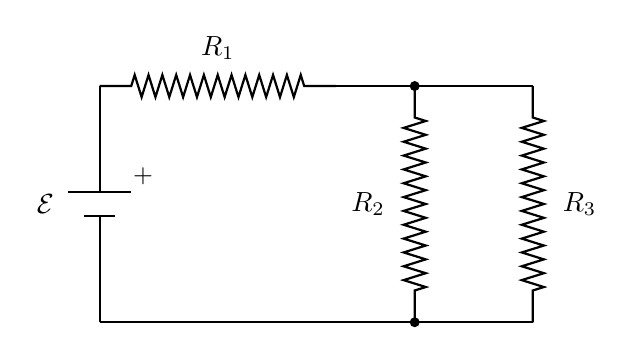
\begin{tikzpicture}[thick, res/.style={decorate,decoration={zigzag,segment length=5pt,amplitude=4pt,pre length=0.4cm,post length=0.4cm}}]
    \draw (0,0) -- (0,1.35);
    \draw (-0.2,1.35) -- (0.2,1.35);
    \draw (-0.4,1.65) -- (0.4,1.65);
    \draw (0,1.65) -- (0,3);
    \node[left] at (-0.45,1.5) {$\mathcal{E}$};
    \node at (0.55,1.85) {\small$+$};
    \draw[res] (0,3) -- (3,3);
    \node[above] at (1.5,3.2) {$R_1$};
    \draw (3,3) -- (5.5,3);
    \draw[res] (4,3) -- (4,0);
    \draw[res] (5.5,3) -- (5.5,0);
    \node[left] at (3.75,1.5) {$R_2$};
    \node[right] at (5.75,1.5) {$R_3$};
    \draw (0,0) -- (5.5,0);
    \fill (4,3) circle (1.8pt); \fill (4,0) circle (1.8pt);
\end{tikzpicture}
\end{center}

\begin{enumerate}[label=\alph*)]
    \item Déterminez la résistance équivalente du circuit.
    \item Déterminez le courant fourni par la pile.
    \item Déterminez le courant qui traverse la résistance $R_2$.
    \item Déterminez la puissance dissipée dans la résistance $R_1$.
\end{enumerate}
